% !TEX root = ElMath_slides_1819.tex
\section{Calculus and nonlinear aspects}

{\bf Motivation:} Optimization and \emph{C}onvolutional \emph{N}eural \emph{N}etwork 

\begin{minipage}[c]{0.88\textwidth}\color{blue}
	\begin{tikzpicture}[->,>=stealth',shorten >=1pt,auto,node distance=2.2cm,
	semithick]
	\node[inner sep=0pt] (dina0) at (7,4)
	{\includegraphics[width=\textwidth]{pics/A_CNN.png}};
	\node (input) at (0,0){Input $x_i$};
	\node (middle) at (7,0){intermediate parameters $q$};
	\node (class) at (13,0){class};
	\node (loss) at (15.5,0){loss $L(x_i,q)$};
	\draw[->] (input) -- (middle);
	\draw[->] (middle) -- (class);
	\draw[->] (class) -- (loss);
	\end{tikzpicture}
\end{minipage}

If we want to identify parameters $q$ which minimize a loss function for specific inputs $x_i$, we have to be able to determine derivatives of a function depending on multiple variables and which itself is a concatenation of multiple intermediate functions.  

\newpage
\gbegin{definition}[Continuous/differentiable]\label{derivative} Let $D\subset\R^m$, $f:D\to \R^n$ and $x_0\in\R^m$ with
$B_\varepsilon(x_0)\subset D$, where $B_\varepsilon(x_0):=\{x\spy \|x-x_0\|_2<\varepsilon\}$ for an $\varepsilon >0$. Then
\ite
\item $f$ is called \emph{\textbf{continuous at $x_0$}}, if $\lim\limits_{n\to \infty}\|f(x_n)-f(x_0)\|_2=0$ for all sequences $\{x_n\}_{n=1}^\infty\subset B_\varepsilon(x_0)$ with the property $\lim\limits_{n\to\infty}\|x_n-x_0\|_2=0$.
\item $f$ is called \emph{\textbf{differentiable at $x_0$}}, if there is a linear mapping $A\in\text{Hom}(\R^m,\R^n)$ such that
\[
\lim_{n\to\infty}\frac{\|(f(x_0)+Ah_n)-f(x_0+h_n)\|_2}{\|h_n\|_2}=0\, , 
\]
for all sequences $\{h_n\}_{n=1}$ with $x_0+h_n\in B_\varepsilon(x_0)$ and $\lim_{n\to\infty}\|h_n\|_2=0$. Since the linear mapping depends on $f$ and $x_0$, we denote it as $Df(x_0):=A$ and call it \emph{(Fréchet) \textbf{derivative}}. 
\eti
\vspace{-0.3cm}
If $f$ is continuous/differentiable at any point $x_0\in D$, we call $f$ continuous/differentiable.
\bend{definition}
%
\vspace{-0.1cm}
{\bf Note} that the definitions are independent of the particular chosen norms $\|.\|$ in finite dimensions. 
%
~\\[0.5cm]
\textbf{How can we recognize continuous/differentiable functions?}
\vspace{-0.2cm}
\ite
\item[$\rightarrow$] Many elementary functions and operations (``+'',``$\cdot$'',trigonometric, etc.) are known to be continuous/differentiable.
\item[$\rightarrow$] Concatenation of continuous/differentiable functions preserves the respective property.
\eti


%\newpage
%\begin{minipage}{0.5\textwidth}
%	\begin{tikzpicture}
%	\node (v2) at (0,2.85) {};
%	\node (v1) at (0,-3.5) {};
%	\node (v3) at (-2.5,-1.5) {};
%	\node (v4) at (4.5,-1.5) {};
%	\draw [-latex] (v1) edge (v2);
%	\draw [-latex] (v3) edge (v4);
%	\draw  plot[smooth cycle, tension=.7] coordinates {(0.5,0) (1.1,1.3) (2.45,1.45) (3,0.5) (3,-1) (1.5,-0.5) (1,-0.5)};
%	\node at (1,2) {$\mathbb{R}^m$};
%	\node at (2.65,0.6) {D};
%	\draw  (1.8,0.25) ellipse (0.7 and 0.7);
%	\node (v5) at (1.85,0) {$x_0$};
%	\node (v6) at (1,0.5) {};
%	\node at (1.5,0.5) {$\epsilon$};
%	\node (v7) at (1.9,0.2) {};
%	\draw  (v7) edge (v6);
%	\draw  (1.9,0.35) ellipse (0.01 and 0.01)[color=red];
%	\draw  (2.05,0.4) ellipse (0.01 and 0.01)[color=red];
%	\draw  (2.2,0.35) ellipse (0.01 and 0.01)[color=red];
%	\draw  (2.35,0.25) ellipse (0.01 and 0.01)[color=red];
%	\node [text=red] at (2.8,-0.15) {$\{x_n\}$};
%	\end{tikzpicture}
%\end{minipage}
%\begin{minipage}{0.5\textwidth}
%	\begin{tikzpicture}
%	\node (v2) at (0,2.85) {};
%	\node (v1) at (0,-3.5) {};
%	\node (v3) at (-2.5,-1.5) {};
%	\node (v4) at (4.5,-1.5) {};
%	\draw [-latex] (v1) edge (v2);
%	\draw [-latex] (v3) edge (v4);
%	\node at (1,2) {$\mathbb{R}^n$};
%	\draw [-latex] plot[smooth, tension=.7] coordinates {(-4,1) (-2.35,1.35) (-0.5,1.05)};
%	\node at (-2.4,1.65) {$f$};
%	\draw [-latex] (1.15,0.6) ellipse (0.05 and 0.05)[color=red,fill=red];
%	\draw [-latex] (0.35,1.15) ellipse (0.05 and 0.05)[color=red,fill=red];
%	\draw [-latex] (1.5,0.15) ellipse (0.05 and 0.05)[color=red,fill=red];
%	\draw [-latex] (0.8,0.95) ellipse (0.05 and 0.05)[color=red,fill=red];
%	\draw [-latex] (1.75,-0.2) ellipse (0.05 and 0.05)[color=black,fill=black];
%	\node at (2.5,0) {$f(x_0)$};
%	\node at (1.85,1.1)[text=red] {$\{f(x_n)\}$};
%	\end{tikzpicture}
%\end{minipage}

% EXAMPLES
\newpage
\begin{bsp} 
	\blank
	continous functions:
	\begin{itemize}
		\item $x \rightarrow x^2, e^x, \sin{x}, \cos{x}, \abs{x} $\\
	\end{itemize}
 ~\\
  differentiable functions:
	\begin{itemize}
		\item $x^2, e^x, \sin{x}, \cos{x}, \ln{x}, e^{-x^2}$\\
		\item $\abs{x}$ is not differentiable! (at $x = 0$)\\
		\item[]
		\begin{tikzpicture}
		\node (v2) at (0,0.5) {};
		\node (v1) at (0,-2.5) {};
		\node (v3) at (-2.5,-1.5) {};
		\node (v4) at (3.1,-1.5) {$x$};
		\draw [-latex] (v1) edge (v2);
		\draw [-latex] (v3) edge (v4);
		\node (v5) at (-1.4,0) {};
		\node (v7) at (1.45,0) {$\mid x \mid$};
		\node (v6) at (0.1,-1.6) {};
		\draw  (v5) edge (v6);
		\node (v8) at (-0.1,-1.6) {};
		\draw  (v8) edge (v7);
		\node (v9) at (-1.15,-1.85) {};
%		\node (v10) at (1.65,-1)[text=\blank] {$ax$};
%		\draw  (v9) edge (v10)[\blank];
		\end{tikzpicture}
	\end{itemize}
\end{bsp}

% MORE EXAMPLES
\newpage
\begin{bsp}
	\blank
	 derivatives
	\begin{itemize}
		\item $f(x) = x^2, \frac{df}{dx}(x) = f^\prime (x) = 2x$\\
		\item $g(x) = e^x, \frac{dg}{dx}(x) = g^\prime (x) = e^x$\\
		\item $h(x) = \ln{x}, \frac{dh}{dx}(x) = h^\prime (x) = \frac{1}{x}$\\
		\item $\rho (x) = \sin{(x)}, \frac{d\rho}{dx}(x) = \rho^\prime (x) = \cos{(x)}$\\
		\item $\psi (x) = \cos{(x)}, \frac{d\psi}{dx}(x) = \psi^\prime (x) = -\sin{(x)}$\\
		\item $f(x) = e^{-x^2}, \frac{df}{dx}(x) = f^\prime (x) = e^{-x^2}\cdot(-2x)$
	\end{itemize}
\end{bsp}
\newpage

\rbegin{theorem}[Differentiable $\Rightarrow$ continuous] Every differentiable function is also continuous, but not vice versa.
\bend{theorem}
\vspace{-0.5cm}
\begin{proof}
	\blank
	If $f$ is differentiable at $x_0$, we observe
	$
	0=\lim_{n\to\infty}\|f(x_0)+Ah_n-f(x_0+h_n)\|_2
	$,
	because otherwise the limit in the definition would not exist. Triangle inequality gives then
	\[
	\lim_{n\to\infty}\|f(x_0)-f(x_0+h_n)\|_2\le \lim_{n\to\infty}\|f(x_0)+Ah_n-f(x_0+h_n)\|_2+\lim_{n\to\infty}\|Ah_n\|_2
	=\lim_{n\to\infty}\|Ah_n\|_2 =0
	\]
	For ``not vice versa'', it is enough to give one counterexample: $\R\ni x\mapsto |x|$.
\end{proof}

\gbegin{definition}[Directional derivative]\label{directional} We assume that $f:\R^m\to\R^n$ is differentiable in $x_0 \in \R^m$ with (Fréchet) derivative $Df(x_0)$ and let $v\in\R^m$. Then, the limit
\[
Gf(x_0)v := \lim_{t\to 0}\frac{f(x_0+tv)-f(x_0)}{t}\ 
\]
exists and it coincides with the Fréchet derivative, i.e., 
$Gf(x_0)v=Df(x_0)v$.
We call $Gf(x_0)v$ the \textbf{directional derivative at $x_0$ in the direction $v$} or \textbf{\emph{G\^ateaux derivative}}.
\bend{definition}
\vspace{0.5cm}
\begin{remark} The G\^ateaux derivative may also exists even if $f$ is not Fr\'echet differentiable (e.g., $x\mapsto |x|$). However, we note that it is a very convenient way to determine analytical derivatives in somewhat confusing situations.
\end{remark}

% EXAMPLES
\newpage
\begin{bsp}
	\blank
	\begin{itemize}
		\item $f(x) = \abs{x}$ is not Fréchet differentiable at 0 but directional derivations exist:\\
		\item[] \begin{tikzpicture}
		\node (v2) at (0,0.5) {};
		\node (v1) at (0,-2.5) {};
		\node (v3) at (-2.5,-1.5) {};
		\node (v4) at (3.1,-1.5) {$x$};
		\draw [-latex] (v1) edge (v2);
		\draw [-latex] (v3) edge (v4);
		\node (v5) at (-1.4,0) {};
		\node (v7) at (1.45,0) {};
		\node (v6) at (0.1,-1.6) {};
		\draw  (v5) edge [thick](v6);
		\node (v8) at (-0.1,-1.6) {};
		\draw  (v8) edge [thick](v7);
		\node (v9) at (-1.15,-1.85) {};
		\end{tikzpicture}\\
		\item[]$Df(x_0)(+1) = {1}$\\
		\item[]$Df(x_0)(-1) = {-1}$\\
	\end{itemize}
\end{bsp}

% MORE EXAMPLES
\newpage
\begin{bsp}
	\blank
	 (for usage of directional derivatives)\\
	\begin{itemize}
		\item[a)]\begin{itemize}
			\item $f: \mathbb{R}^n \rightarrow \mathbb{R}, x \rightarrow x^\top x$\\
			\item[]$Df(x)v = \frac{d}{dt}\bigg|_{t=0}f(x+tv) = \frac{d}{dt}\bigg|_{t=0} [(x+tv)^\top (x+tv)] =$ \\
			\item[] $=\frac{d}{dt}\bigg|_{t=0}[x^\top x+x^\top (tv) +(tv)^\top(tv)] = \frac{d}{dt}\bigg|_{t=0}[x^\top x + 2tx^\top v + t^2 v^\top v] =$\\
			\item[] $=\underbrace{\frac{d}{dt}\bigg|_{t=0} (x^\top x)}_{0} + \underbrace{\frac{d}{dt}\bigg|_{t=0} (2tx^\top v)}_{2x^\top v} + \underbrace{\frac{d}{dt}\bigg|_{t=0}(t^2 v^\top v)}_{(2tv^\top v)\bigg|_{t=0} = 0}$\\
			\item[]$= 2x^\top v = Df(x)v \Rightarrow Df(x) = 2x^\top$
		\end{itemize}
		\item[b)] \begin{itemize}
			\item $f(x) = x^\top Ax$, A symmetric positive definit\\
			\item[] $Df(x)v = \frac{d}{dt}\bigg|_{t=0}f(x+tv) = \frac{d}{dt}\bigg|_{t=0} [(x+tv)^\top A(x+tv)] =$ \\
			\item[] $=\frac{d}{dt}\bigg|_{t=0}[x^\top Ax+2tx^\top Av + t^2 v^\top Av] =$\\
			\item[] $ = 2x^\top Av \Rightarrow Df(x) = 2x^\top A = 2(Ax)^\top$\\
		\end{itemize}
		\item[c)] \begin{itemize}
			\item $f(A) = A^{-1}$, $A \in$ GL $(n,\mathbb{R})$\\
			\item[] observe: $(A+tH)^{-1} (A+tH) = I, \forall{t}$\\
			\item[] $\Rightarrow \frac{d}{dt}\bigg|_{t=0}(A+tH)^{-1} A + A^{-1} \overbrace{\frac{d}{dt}\bigg|_{t=0}(A+tH)}^{H} = 0$\\
			\item[] $\Rightarrow Df(A)H = \frac{d}{dt}\bigg|_{t=0}(A+tH)^{-1} = -A^{-1}HA^{-1}$
		\end{itemize}
	\end{itemize}
\end{bsp}

%%%
\newpage
~\\[-0.8cm]
For notational ease, the directional derivative in direction of the standard basis vectors is given a special name:\\[-0.5cm]
\gbegin{definition}[Partial derivative]
Let $f:\R^m\supset D\to\R^n$ be differentiable in $x_0\in D$.  we define the so-called \emph{\textbf{partial derivative of $f$ at $x_0$}} with respect to the $j$-th variable by
\[
\frac{\partial }{\partial x_j}f(x_0):=\frac{\partial f}{\partial x_j}(x_0):=Df(x_0)e_j
\]
where $e_i$ is the $j$-th standard basis vector.
\bend{definition}
%
Since $Df(x_0)$ is a linear mapping, we can represent it by a matrix. 
\rbegin{lemma}[Jacobian] Let $f:\R^m\supset D\to\R^n$ be differentiable in $x_0\in D$ with derivative $Df(x_0)\in\text{Hom}(\R^m,\R^n)$. Then, the so-called \emph{\textbf{Jacobian matrix}}
\[\small
J(x_0):=\bbmat
\frac{\partial f_1}{\partial x_1}(x_0)&\ldots&\frac{\partial f_1}{\partial x_m}(x_0)\\
\vdots& &\vdots\\
\frac{\partial f_n}{\partial x_1}(x_0)&\ldots&\frac{\partial f_n}{\partial x_m}(x_0)
\ebmat
\]
is the matrix representation of $Df(x_0)$ with respect to the standard bases.
\bend{lemma}
\vspace{-0.5cm}
\begin{proof}
	\blank
	The $j$-th column of the matrix representation of $Df(x_0)$ is given by $Df(x_0)e_j$ expressed in the canonical bases, which gives
	\vspace{-0.5cm}
	\[
	J(x_0)e_j=Df(x_0)e_j=\frac{\partial f}{\partial x_j}(x_0)=
	\bbmat
	\frac{\partial f_1}{\partial x_j}(x_0)\\ \vdots \\ \frac{\partial f_n}{\partial x_j}(x_0)
	\ebmat.
	\]
	~\\[-0.5cm]
\end{proof}


\newpage
In the special case that $n=1$, i.e., $f\colon \R^m \to \R$, the Jacobian matrix is only consisting of one row, i.e., is a vector in $\R^m$, given by
$$J(x_0) = \left[\frac{\partial f}{\partial x_1}(x_0), \ldots,\frac{\partial f}{\partial x_m}(x_0) \right] = \nabla f(x_0)^T  $$
which we call the \textbf{\color{defgruen}gradient of $f$ at $x_0$}. Note that the gradient is usually defined to be a column vector.
\begin{bsp} 
	\blank
	Why convenient to only compute partial derivatives? (any vector can be expressed in the standard basis)\\[-1cm]
	\begin{itemize}
		\item[a)] \begin{itemize}
			\item[] $f(x_1,x_2) := \begin{bmatrix}
			x_2 \cdot \cos{(x_1)}\\
			x_1 \cdot \sin{(x_2)}\\
			\end{bmatrix} := \begin{bmatrix}
			f_1(x_1,x_2)\\
			f_2(x_1,x_2)
			\end{bmatrix}$\\
			\item[] $J(x_1,x_2) = \begin{bmatrix}
			\frac{\partial f_1}{\partial x_1} & \frac{\partial f_1}{\partial x_2}\\
			\frac{\partial f_2}{\partial x_1} & \frac{\partial f_2}{\partial x_2}
			\end{bmatrix} = \begin{bmatrix}
			-x_2\sin{(x_1)} & \cos{x_1}\\
			\sin{(x_2)} & x_1 \cos{(x_2)}
			\end{bmatrix}$
		\end{itemize}
		\item[b)]\begin{itemize}
			\item[] $f(x) = x^\top x = x_1^2 + x_2^2 + \cdots + x_n^2 \in \mathbb{R}$\\
			\item[] $J(x_1,\cdots,x_n) = [\frac{\partial f}{\partial x_1}, \frac{\partial f}{\partial x_2}, \cdots, \frac{\partial f}{\partial x_n}] = [2x_1,2x_2,\cdots, 2x_n] = 2\cdot[x_1,\cdots,x_n]=2x^\top$
		\end{itemize}
	\end{itemize}
\end{bsp}
%
%
\newpage
Derivative of concatenated functions:
\rbegin{theorem}[Chain rule] \label{chain}Consider mappings $g:\R^\ell\supset D_g\to D_f\subset\R^m$ differentiable in $x_0\in D_g$ with Jacobian $J_g(x_0)$ and $f:\R^m\supset D_f\to \R^n$, differentiable in $g(x_0)\in D_f$ with Jacobian $J_f(g(x_0))$. Then, the concatenation is differentiable with Jacobian $J_{f\circ g}(x_0)$ and
\[
D(f\circ g)(x_0)=Df(g(x_0))\circ Dg(x_0)\text{~~~and~~~}
\boxed{J_{f\circ g}(x_0)=J_f(g(x_0))\cdot J_g(x_0)}.
\]
\bend{theorem}
%\begin{proof} Standard result.
%\end{proof}

%
A special case:
\rbegin{corollary}Consider with the assumptions of Theorem \ref{chain} for the special case $\ell=1$. Then
\[
\frac{d (f\circ g)}{d t}(t_0):=D(f\circ g)(t_0)=\sum_{i=1}^m\frac{\partial f}{\partial x_i}(g(t_0))\cdot g_i^\prime(t_0)
\]
\bend{corollary}
\begin{proof}
	\blank 
	As it is going to happen later on as well, we are now mixing up Jacobians with derivatives and observe as preparation for the chain rule
	\[
	J_f(g(t))=\left[\frac{\partial f}{\partial x_1}(g(t)),\ldots,\frac{\partial f}{\partial x_m}(g(t))\right]\, , \qquad
	J_g(t)=\bbmat
	g_1^\prime(t)\\ \vdots \\g_m^\prime(t)
	\ebmat
	\] 
\end{proof}

\begin{bsp}
	\blank
	\begin{itemize}
		\item $f(t) = \rho(t,g(t)), \hspace{0.5cm} \rho: \left(\begin{array}{c}
		x_1\\
		x_2
		\end{array}\right) \rightarrow r\in \mathbb{R}$\\
		\item[] $f^\prime(t_0) = \frac{\partial\rho}{\partial x_1} (t_0,g(t_0)) + \frac{\partial\rho}{\partial x_2} (t_0,g(t_0))\cdot g^\prime (t_0)$
	\end{itemize}
\end{bsp}
\newpage




% TAYLOR
\rbegin{lemma}[Taylor approximation]\label{taylor}
Let $f:\R^n\supset B_\varepsilon(\hat{x})\to\R^n$ be differentiable at $\hat{x}$ with some $\varepsilon>0$. Assume further that there is a (Lipschitz) constant $L \geq 0$ such that the Jacobian  $J$
satisfies
\begin{align}
 \|J(y)-J(x)\|\le L\|y-x\|\, ,\quad\forall x,y\in B_\varepsilon(\hat{x}). \label{lipschitz}
\end{align}
Then, there holds
$$
\|f(y)-\left[f(x)+J(x)(y-x)\right]\|\le \frac{L}{2}\|y-x\|^2\, ,\quad\forall x,y\in B_\varepsilon(\hat{x})
$$
which we rephrase with the notation:
$$
f(y)=f(x)+J(x)(y-x) + \mathcal{O}(\|y-x\|^2).
$$
\bend{lemma}
%\begin{proof} Standard proofs require the major theorem of calculus, where we need integration, cf.~definition \ref{def-integral}.
%\end{proof}
%NEWTON_KANTOROVICH
\rbegin{theorem}[simplified Newton-Kantorovich]
Let $f:\R^n\supset B_\varepsilon(\hat{x})\to\R^n$ be differentiable with invertible derivative for some $\varepsilon>0$ and $f(\hat{x})=0$. Assume the Lipschitz condition \eqref{lipschitz} and the existence of an upper bound $\|J(x)^{-1}\|<M$ for some $M<\infty$ and for all $x\in B_\varepsilon(\hat{x})$. Then, the Newton iteration
\[
\boxed{x^{k+1}:=x^k+\Delta x^k\, , \text{~ where~ }\Delta x^k\text{~ solves~ }f(x^k)+J(x^k)\Delta x^k=0}
\]
converges quadratically to $\hat{x}$, provided $x^1$ is chosen sufficiently close to $\hat{x}$, i.e.
\[
\|x^{k+1}-\hat{x}\|\le c \|x^{k}-\hat{x}\|^2\, ,\quad c<\infty.
\]
\bend{theorem}
%{\bf Proof:} This is a simplified version of the Newton-Kantorovich theorem which has less strict assumptions but whose formulation is much more involved. The original version of Newton-Kantorovich not only shows quadratic convergence but also states conditions, under which a locally unique root for $f$ exists as the Cauchy limit of the Newton sequence. \bewende

% REMARKS and EXAMPLES
\newpage
{
%
	\blank
	\begin{itemize}
		\item Lemma 11.8 is a small n-dim version of the Taylor series $f: \mathbb{R}\rightarrow \mathbb{R}$, which can be arbitrary often differentiated in $\hat{x}$\\
		\item[] then $f(y) = \sum\limits_{k=0}^\infty \frac{1}{k!} f^{(k)}(\hat{x})(y-\hat{x})^k$\\
		\item Example: $f(x) = e^x, f^\prime (x) = e^x, f^{(k)} (x) = e^x$\\
		\item[] choose $\hat{x} = 0 \Rightarrow e^{\hat{x}}=1 \Rightarrow f(y) = \sum\limits_{k=0}^\infty \frac{1}{k!} g^k$\\
		\item[] $g(x) = e^{2x}, g(0) = 1, g^\prime(0) = 2e^{2\cdot 0}=2, g^{\prime\prime} (0) = 2\cdot 2 \cdot e^{2\cdot 0}= 2^2 \Rightarrow g^{(k)} (0) = 2^k$\\
		\item[] $g(y) = \sum\limits_{k=0}^\infty \frac{1}{k!} 2^k y^k = \sum\limits_{k=0}^\infty \frac{1}{k!} (2y)^k$
	\end{itemize}
%
\newpage
Idea of Newton iteration:\\
	\begin{itemize}
		\item start at x, try to find step $\Delta x$ torwards solution $\hat{x}$ with $f(\hat{x})=0$\\
		\item[] $f(x+\Delta x) = \underbrace{f(x) + J(x))\Delta x}_{\text{want 0 here}} + O(\norm{\Delta x}^2)$\\
		\item[] i. e. $\Delta x$ solves $J(x)\Delta x = -f(x)$ then step $x^{\text{new}} = x + \Delta x$
	\end{itemize}
}

%HERON METHOD AS NEWTON
\newpage
{\bf Example: Heron method} \\[0.5cm]
Determine the root of $f(x):=x^2-2$ for $x\in\R$:
\ite
\item[] We have $f(x^k)+J(x^k)\Delta x^k=(x^k)^2-2+2x^k\Delta x^k$
\item[] $\Rightarrow \Delta x^k=-\frac{(x^k)^2-2}{2x^k}=-\frac{x^k}{2}+\frac{1}{x^k}$
\item[] $\Rightarrow x^{k+1}:=x^k+\Delta x^k=x^k-\frac{x^k}{2}+\frac{1}{x^k}=\frac12\left(x^k+\frac{2}{x^k}\right)$ ~~~~(Heron method (cf.~section \ref{realnumbers}))
\item[] $\rightarrow$ Now, we can truly understand, why Heron's method works so well!
\eti
\vspace{1cm}
\begin{remark} In many cases, Newton's method does not work right out of the box, because the starting vector $x^1$ is too far away from the solution. Then, techniques for adaptive step-length reduction (damping, relaxation, line-search) have to be used in order to enforce convergence. Details of these approaches fill multiple books. When Newton's method works, i.e., after an initial damped phase, it gets one blazingly fast in a matter of roughly 5 iterations to the solution up to machine accuracy.
\end{remark}


%Newton example system of three equations:
%f1(x, y, z) = log(x) + exp(-x*y) - exp(-2)
%f2(x, y, z) = exp(x) - sqrt(z)/x - exp(1) + 2
%f3(x, y, z) = x + y - y*z + 5
%You can verify that the value (x, y, z)=(1, 2, 4) is an exact root of this system.
%
%start with (1,1,1)

\begin{minipage}[c]{0.6\textwidth}
	\lstinputlisting[lastline=5]{python_examples/A_newton.py}
	\vspace{-0.25cm}
	\centerline{\vdots}
	\vspace{-0.25cm}
	\lstinputlisting[firstline=13,firstnumber=13,lastline=13]{python_examples/A_newton.py}
	\vspace{-0.25cm}
	\centerline{\vdots}
	\vspace{-0.25cm}
	\lstinputlisting[firstline=27,firstnumber=27]{python_examples/A_newton.py}
\end{minipage}
\begin{minipage}[c]{0.05\textwidth}
\end{minipage}
\begin{minipage}[c]{0.35\textwidth}
	{\bf Newton example in 3D}
	\begin{align*}
	f(x,&y,z)=\\
	&\bbmat
	\log(x) + e^{-x\cdot y} - \frac{1}{e^2}\\
	e^{x} - \frac{\sqrt{z}}{x} - e + 2.0\\
	x + y - y\cdot z + 5.0
	\ebmat
	\end{align*}
	solution vector: $[1,2,4]^\top$
	
	start vector: $1.5\cdot[1,1,1]^\top$
	
	\begin{verbatim}
	it  0, res =6.47e+00
	it  1, res =3.37e+00
	it  2, res =2.71e-01
	it  3, res =2.48e-02
	it  4, res =1.93e-05
	it  5, res =1.20e-11
	it  6, res =8.89e-16
	it  7, res =0.00e+00
	it  8, res =0.00e+00
	it  9, res =0.00e+00
	\end{verbatim}
	
	Comparison with {\tt optimize.root} method from {\tt scipy}.
	
	\vspace{0.25cm}
	
\end{minipage}


\newpage
\subsection{Essentials of back propagation}

\emph{Simple first example:} Consider concatenated differentiable functions $f\circ g(x)$ written in the seemingly complicated form with intermediate variable $z$:
\[
f(z)\text{ , where }z-g(x)=0 
\]
Thus, $z$ is a function of $x$, namely $z(x)=g(x)$. Thus,
\[
f\circ g(x)\equiv\LL(x,\lambda):= f(z(x))+\lambda^\top(z(x)-g(x))\, ,
\text{ for any }\lambda.
\]
Now,
\begin{align*}
\frac{d(f\circ g)(x)}{dx}&=
\frac{\partial \LL(x,\lambda)}{\partial x}=
\frac{df}{dz}\frac{dz}{dx}+\lambda^\top\left(\frac{dz}{dx}-\frac{dg}{dx}\right)\\
&=\left(\frac{df}{dz}+\lambda^\top\right)\frac{dz}{dx}-\lambda^\top\frac{dg}{dx}
\end{align*}
Thus, $d(f\circ g)/dx$ can be determined in two steps (note that $\lambda$ can be chosen arbitrarily)
\ite
\item[(1)] $\lambda:=-\left(\frac{df}{dz}(z(x))\right)^\top$
\item[(2)] $\frac{d(f\circ g)(x)}{dx}=-\lambda^\top\frac{dg}{dx}(x)
$
\eti

These two steps are just a more complicated formulation of the chain rule, but this Lagrangian principle is the foundation of the backward mode of automatic differentiation and also of the back propagation in ANN, as we'll see now.

\emph{Abstract back propagation:}
We consider the concatenation
\begin{align*}
h(w_N,\ldots, w_1,x):=&f(g_N(w_N,(g_{N-1}(w_{N-1},(\ldots ,g_1(w_1,x))\ldots ))))\\
=&f\circ g_{N}(w_{N},\cdot)\circ g_{N-1}(w_{N-1},\cdot)\circ\cdots
\circ g_{1}(w_{1},x)
\end{align*}
illustrated by the diagramm:

\hspace{0.5cm}
\begin{tikzpicture}[->,>=stealth',shorten >=1pt,auto,node distance=2.2cm,
semithick]
\node (input) at (0,0){$x$};
\node (g1) at (2,0){\fbox{$g_{1}$}};
\node (w1) at (2,-1.5){$w_1$};
\node (z1) at (4,0){$z_{1}$};
\node (gNm1) at (7,0){\fbox{$g_{N-1}$}};
\node (wNm1) at (7,-1.5){$w_{N-1}$};
\node (zNm1) at (9.25,0){$z_{N-1}$};
\node (gN) at (11.25,0){\fbox{$g_N$}};
\node (wN) at (11.25,-1.5){$w_N$};
\node (zN) at (13.25,0){$z_N$};
\node (fz) at (15.25,0){$f(z_N)$};
\draw[->] (input) -- (g1);
\draw[->] (w1) -- (g1);
\draw[->] (g1) -- (z1);
\draw[->, dotted] (z1) -- (gNm1);
\draw[->] (wNm1) -- (gNm1);
\draw[->] (gNm1) -- (zNm1);
\draw[->] (zNm1) -- (gN);
\draw[->] (wN) -- (gN);
\draw[->] (gN) -- (zN);
\draw[->] (zN) -- (fz);
\end{tikzpicture}


Again, this can be written in the fashion
\[
h(w_N,\ldots, w_1,x)=f(z_{N})\text{ ,~ where~ }z_k-g_k(w_k,z_{k-1})=0\, , ~~~k=1,\ldots,N\, , ~~z_0:=x
\]
Again
\[
h(w_N,\ldots, w_1,x)\equiv
\LL(w,x,\lambda):=f(z_N)+\sum_{k=1}^N\lambda_k^\top(z_k-g_k(w_k,z_{k-1}))\, ,
\text{~~ for any }\lambda_k
\]
Thus
\begin{align*}
\frac{dh}{dw_i}&=\frac{df}{dz}\frac{dz_N}{dw_i}+
\sum_{k=i}^N\lambda_k^\top\frac{dz_k}{dw_i}-\sum_{k=i+1}^N\lambda_k^\top\frac{\partial g_k}{\partial z}\frac{\partial z_{k-1}}{\partial w_i} -\lambda_i^\top\frac{\partial g_i}{\partial w_i}\\
&=\frac{df}{dz}\frac{dz_N}{dw_i}+
\sum_{k=i}^N\lambda_k^\top\frac{dz_k}{dw_i}-\sum_{k=i}^{N-1}\lambda_{k+1}^\top\frac{\partial g_{k+1}}{\partial z}\frac{dz_{k}}{dw_i} -\lambda_i^\top\frac{\partial g_i}{\partial w_i}\\
&=\left(\frac{df}{dz}+\lambda_N^\top\right)\frac{dz_N}{dw_i}+
\sum_{k=i}^{N-1}\left(\lambda_k^\top-\lambda_{k+1}^\top\frac{\partial g_{k+1}}{\partial z}\right)\frac{dz_{k}}{dw_i} -\lambda_i^\top\frac{\partial g_i}{\partial w_i}.
\end{align*}
Thus, if the $\lambda$'s satisfy the recursion
\[
\lambda_N=-\left(\frac{df}{dz}(z_N)\right)^\top\, ,\ 
\lambda_k=\left(\frac{\partial g_{k+1}}{\partial z}(w_{k+1},z_k)\right)^\top \lambda_{k+1}\, ,\qquad 
k=N-1,N-2,\ldots, i
\]
we achieve the expression
\[
\frac{dh}{dw_i}(w_N,\ldots, w_1,x)= -\lambda_i^\top\frac{\partial g_i}{\partial w_i}(w_i,z_{i-1}).
\]

\begin{remark}
	The technique presented is an example of a fairly general principle for the derivation of iterations towards complicated derivatives. This principle is used in the backward mode of automatic differentiation and in the derivation of adjoint equations for optimization problems involving differential equations.
\end{remark}



\section{Integration and quadrature}

Quadrature = numerical approximation of an integral  

Here, we do not go very deep into the foundations, but rather use the following operational definition. A more detailed view is required for measure and probability theory.
\gbegin{definition}\label{def-integral} ~\\[-0.7cm]
\ite
\item[(1D)] For the interval $[a,b]$ with $-\infty< a\le b<\infty$ and an (integrable) function $f:[a,b]\to\R$, we define
\[
\int_a^bf(x)dx:=F(b)-F(a)=:[F(x)]_a^b\, , \text{ where } F:[a,b]\to\R \text{ satisfies } F'(x)=f(x) 
\]
If instead $f:[a,b]\to\R^k$, this definition is applied to each component $f_i(x)$ separately.
\item[(nD)] Consider a domain $D:=\mathop{\times}_{i=1}^n[a_i,b_i]$  with $-\infty< a_i\le b_i<\infty$ and an (integrable) function $f:D\to\R^k$. We define
\[
\int_D f(x)dx:=\int_{a_1}^{b_1}\int_{a_2}^{b_2}\ldots\int_{a_n}^{b_n}
f(x_1,x_2,\ldots,x_n)dx_n\ldots dx_2dx_1
\]
\eti
If $a,b$ or $a_i,b_i$ are not finite or if $f$ is not finite there, one has to use appropriate limits. A function $f$ is called \textbf{integrable}, if the expressions defined above are well defined and finite. Countably many points on $\R$ are considered zero sets and integrals over them are zero per definition.
\bend{definition}
\newpage 
{
\blank
\small
~ \\[-1.5cm]
\begin{bsp} 
	\begin{itemize}
		\item[a)] \[\int\limits_0^1 x^3 dx = [\frac{x^4}{4}]_0^1 = \frac{1}{4}\]   \\[-0.9cm]
		\item[b)] \[\int_D \norm{x}^2 dx = \int_{[0,1]^2} x^\top x dx = \int_0^1 \int_0^1 (x_1^2 +x_2^2) dx_1 dx_2 = 
	   \int_0^1 [\frac{x_1^3}{3} + x_1 x_2^2]_0^1 dx_2 = \int_0^1 \frac{1}{3} + x_2^2 dx_2 = [\frac{x_2}{3} + \frac{x_2^3}{3}]^1_0 = \frac{1}{3}+\frac{1}{3} = \frac{2}{3}\]
	\end{itemize}
\end{bsp}
\textbf{Substitution rule in 1d} \vspace{-0.5cm}
\begin{itemize}
	\item[] \[ \int_a^b f(x) dx,\; \text{let}\; x = g(y) \Rightarrow \frac{dx}{dx} = g^\prime (y) \Rightarrow dx = g^\prime (gy) dy \]
	\item[] \[ \Rightarrow \exists \alpha,\beta \; \text{with}\; a=g(\alpha), b= g(\beta): \hspace{0.5cm} \int_a^b f(x) dx = \int_\alpha^\beta f(g(y))g^\prime (y) dy \]
\end{itemize}
\begin{bsp}
	\begin{itemize}
		\item[] \[ \int_{1/50}^2 \frac{e^{\frac{2}{y}}}{y^2}dy, \; \text{let}\; x := \frac{2}{y} = 2\cdot y^{-1}\]
		\item[] \[ \Rightarrow \frac{dx}{dy} = - \frac{2}{y^2} \Rightarrow \frac{1}{y^2} dy = - \frac{dx}{2} \; \text{and} \; a = \frac{2}{1/50} = 100, b= \frac{2}{2} = 1\]
		\item[] \[ \Rightarrow \int_{1/50}^2 \frac{e^{\frac{2}{y}}}{y^2}dy = \int_{1/50}^2 e^{\frac{2}{y}} \underbrace{\frac{1}{y^2}dy}_{-\frac{dx}{2}} = \int_100^1 - \frac{e^x}{2}dx = -\frac{1}{2}(e^1 - e^{100}) = \frac{e^{100}-e^1}{2}\]
	\end{itemize}
\end{bsp}
}


\newpage
{
	\blank
\textbf{Substitution rule in nD:}
\begin{itemize}
	\item[] \[ \int_D f(x)dx, \; \text{let}\; x=g(y), g \; \text{invertible (on image) and} \]
	\item[] \[ D = g(E) \Rightarrow dx = \sqrt{\det(Dg(y)^\top Dg(y))}dy\] 
	\item[] \[ \int_D f(x)dx = \int_E f(g(y))\sqrt{\det(Dg(y)^\top Dg(y))}dy\]
\end{itemize}
\begin{bsp}
	\begin{itemize}
		\item[a)]\begin{itemize}
			\item[] $\left(\begin{array}{c}
			x_1\\
			x_2
			\end{array}\right) = g \left(\begin{array}{c}
			r\\
			\phi
			\end{array}\right) = \left(\begin{array}{c}
			r \cos{\phi}\\
			r \sin{\phi}
			\end{array}\right)$\\
			\item[] $Dg = \begin{bmatrix}
			\frac{\partial g_1}{\partial r} & \frac{\partial g_1}{\partial \phi}\\
			\frac{\partial g_2}{\partial r} & \frac{\partial g_2}{\partial \phi}
			\end{bmatrix} = \begin{bmatrix}
			\cos{\phi} & -r\sin{\phi} \\
			\sin{\phi} & r\cos{\phi}
			\end{bmatrix}$\\
			\item[] $\abs{\det(Dg)} = \abs{\cos{\phi r}\cos{\phi} - \sin{\phi}(-r\sin{\phi})} = \abs{r(\cos{\phi}^2 + \sin{\phi}^2)} = r$\\
			\item[] Area of D = \[ \int_D 1dx = \int_E 1\abs{\det(Dg(r,\phi))}d(r,\phi) = \int_o^\pi \int_1^2 rdrd\phi = \frac{3}{2}\pi\]
		\end{itemize}
		\item[b)] Surface of the unit ball\\
%		\begin{tikzpicture}[line cap=round, line join=round]
%		\clip(-2.19,-2.49) rectangle (2.66,2.58);
%		\draw(0,0) circle (2cm);
%		\draw [rotate around={0.:(0.,0.)},dash pattern=on 3pt off 3pt] (0,0) ellipse (2cm and 0.9cm);
%		\draw [->] (0,0) -- (0,2);
%		\draw [->] (0,0) -- (-0.81,-0.79);
%		\draw [->] (0,0) -- (2,0);
%		\draw (-1.2,-0.75) node[anchor=north west] {$\mathbf {\hat{x}}$};
%		\draw (2.07,0.3) node[anchor=north west] {$\mathbf {\hat{y}}$};
%		\draw (-0.27,2.6) node[anchor=north west] {$\mathbf {\hat{z}}$};
%		\scriptsize
%		\end{tikzpicture} 
		 \begin{itemize}\small
			\item[] $\left(\begin{array}{c}
			x\\
			y\\
			z
			\end{array} \right) g(\phi,\theta), \hspace{1cm}0 \leq \theta \leq \frac{\pi}{2}, 0 \leq \phi \leq \frac{\pi}{2}$\\
			\item[] $g(\phi,\theta) = \left(\begin{array}{c}
			\cos{\phi}\cos{\theta}\\
			\sin{\phi}\sin{\theta}\\
			\sin{\theta}
			\end{array}
			\right)$\\
			\item[] $Dg = \begin{bmatrix}
			-\sin{\phi}\cos{\theta} & -\cos{\phi}\sin{\theta}\\
			\cos{\phi}\cos{\theta} & -\sin{\phi}\sin{\theta}\\
			0 & \cos{\theta}
			\end{bmatrix} \in \mathbb{R}^{3\times2}$\\
			\item[] $\sqrt{\det(Dg(\phi,\theta)^\top Dg(\phi,\theta)} = \cdots = \cos{\theta}$\\
			\item[] \[\int_0^1 1 dA = \int_E 1\sqrt{\det(Dg(\phi,\theta)^\top Dg(\phi,\theta))}d\theta d\phi\]
			\item[] \[ = \int_0^{\frac{\pi}{2}}\int_0^{\frac{\pi}{2}} \cos{\theta}d\theta d\phi = \int_0^{\frac{\pi}{2}}\underbrace{[\sin{\theta}]_0^{\frac{\pi}{2}}}_{1} d\phi = \frac{\pi}{2}\] 
			\item[] Total surface of unitball = $8 \cdot \abs{0} = 8\cdot \frac{\pi}{2} = 4\pi$
		\end{itemize}
	\end{itemize}
\end{bsp}
}

\newpage
{\bf Idea of numerical integration, aka quadrature:} approximate the function to be integrated piecewise by simple functions, for which the integral is given analytically.

Example: trapezoidal rule:

\pgfplotsset{
	integral axis/.style={
		axis lines=middle,
		enlarge y limits=upper,
		axis equal image, width=12cm,
		xlabel=$x$, ylabel=$y$,
		ytick=\empty,
		xticklabel style={font=\small, text height=1.5ex, anchor=north},
		samples=100
	},
	integral/.style={
		domain=2:10,
		samples=9
	},
	integral fill/.style={
		integral,
		draw=none, fill=#1,
		%on layer=axis background
	},
	integral fill/.default=cyan!10,
	integral line/.style={
		integral,
		very thick,
		draw=#1
	},
	integral line/.default=black
}

\hspace{2cm}
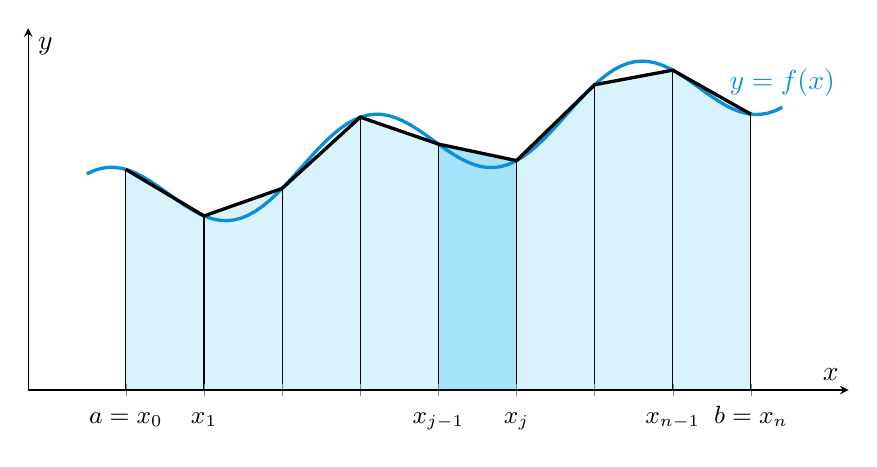
\begin{tikzpicture}[
% The function that is used for all the plots
declare function={f=x/5-cos(deg(x*1.85))/2+2;}
]
\begin{axis}[
integral axis,
ymin=0,
xmin=0.75, xmax=11.25,
domain=1.5:10.4,
xtick={2,...,10},
xticklabels={$a=x_0$, $x_1$,,,$x_{j-1}$,$x_j$,,$x_{n-1}$,$b=x_n$},
axis on top
]
% The filled area under the approximate integral
\addplot [integral fill=cyan!15] {f} \closedcycle;

% The highlighted segment
\addplot [integral fill=cyan!35, domain=6:7, samples=2] {f} \closedcycle;

% The function
\addplot [very thick, cyan!75!blue] {f} node [anchor=south] {$y=f(x)$};

% The approximate integral
\addplot [integral line=black] {f};

% The vertical lines between the segments
\addplot [integral, ycomb] {f};

\end{axis}
\end{tikzpicture}
\begin{align*}
\int_{x_{j-1}}^{x_j}f(x)dx\approx\int_{x_{j-1}}^{x_j}\frac{x_{j-1}-{\color{red}x}}{x_j-x_{j-1}}
\cdot f(x_{j-1})+\frac{{\color{red}x}-x_{j-1}}{x_j-x_{j-1}}
\cdot f(x_{j})d{\color{red}x}=(x_j-x_{j-1})\cdot\frac{f(x_{j-1})+f(x_{j})}{2}
\end{align*}
Thus, for constant distances $x_j-x_{j-1}\equiv h:=(b-a)/n$, we obtain
\[
\int_a^bf(x)dx=\frac{f(a)+f(b)}{2}+\sum_{i=1}^{n-1}h\cdot f(x_i)+\mathcal{O}(h^2) 
\]
This can be generalized to higher order polynomials, as well as, to higher dimensions.

\begin{minipage}[c]{0.6\textwidth}
	\lstinputlisting{python_examples/A_integration.py}
\end{minipage}
\begin{minipage}[c]{0.05\textwidth}
\end{minipage}
\begin{minipage}[c]{0.35\textwidth}
	{\bf Quadrature example:}
	
	\bigskip
	Approximate
	\[
	\int_{-2}^2e^{-x^2}dx=\sqrt{\pi}\cdot\text{erf}(2)
	\]
	
	Approximation by trapezoidal rule, general quadrature and comparison with erf.
	\begin{verbatim}
	1.7640408807911219
	1.764162781524843
	1.764162781524843
	\end{verbatim}
	
	Note that the integral cannot be evaluated analytically.
	
	\vspace{0.25cm}
	
\end{minipage}
